%%%%%%%%%%%%%%%%%%%%%%%%%%%%%%%%%%%%%%%%%%%%%%%%%%%%%%%%%%%%%%%%%%%%
\section{Slow Controls}
\label{sec:fddp-slow-cryo-ctrl}

% same for SP and DP

The slow controls system collects, archives, and displays data from
a broad variety of sources, and provides real time alarms and
warnings for detector operators. Data is acquired via network
interfaces.  Figure \ref{fig:gen-slow-controls-diagram} shows the
connections between major parts of the slow controls system and other
systems.  %The following subsections describe the required hardware and
%software for the slow controls.

\begin{dunefigure}[Slow Controls connections and data]{fig:gen-slow-controls-diagram}
{Typical Slow Controls system connections and data flow}
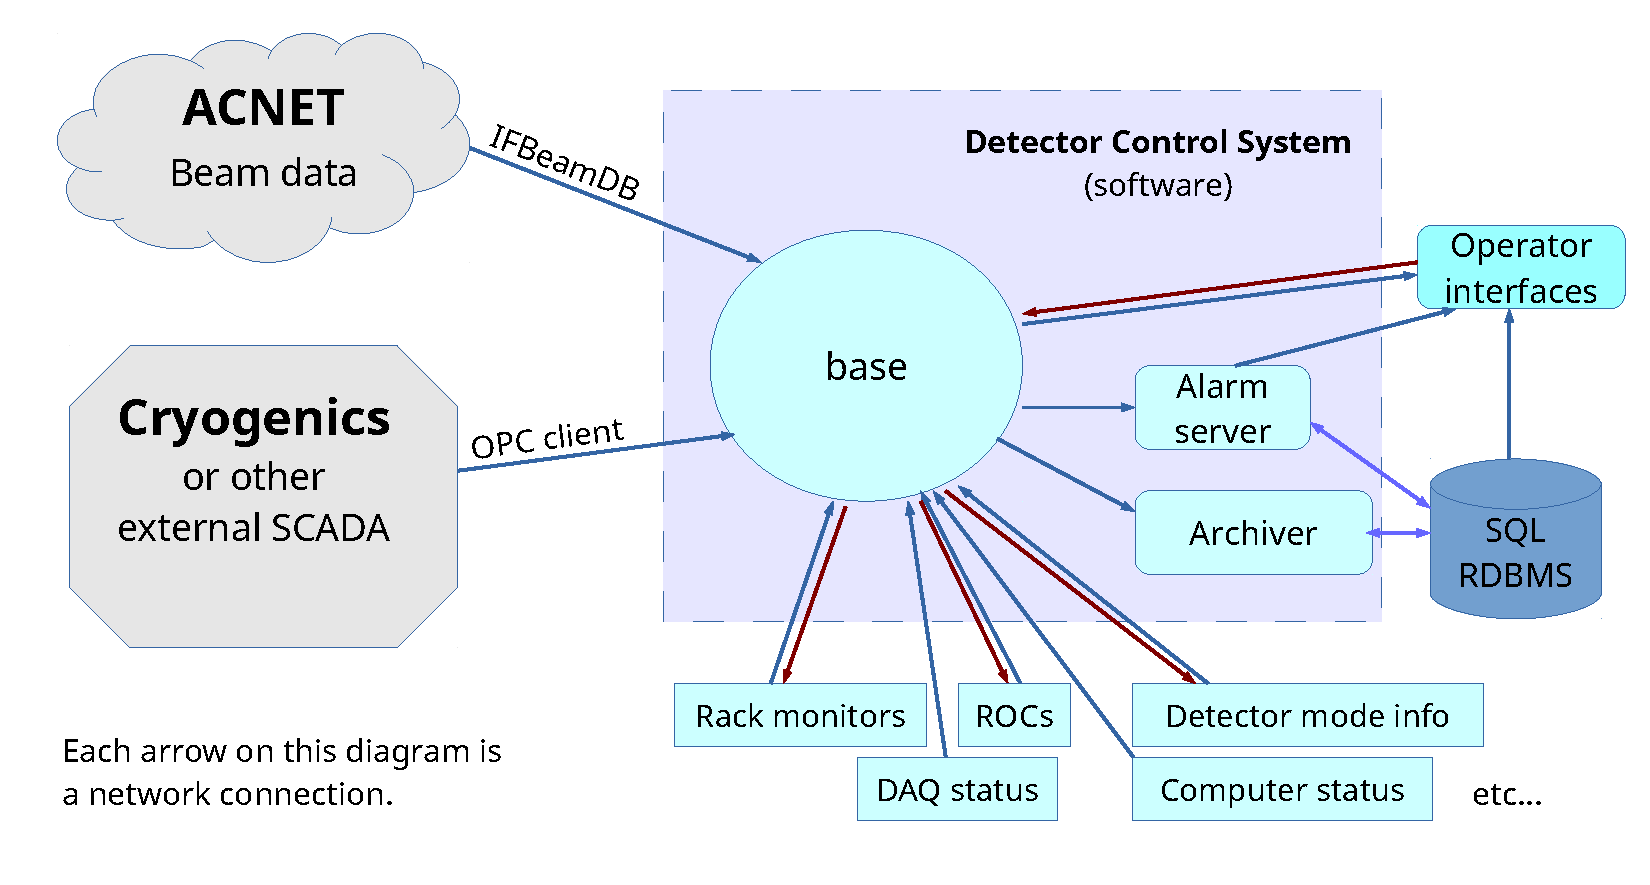
\includegraphics[width=0.7\textwidth]{slow-controls-diagram}
\end{dunefigure}





%%%%%%%%%%%%%%%%%%%%%%%%%%%%%%%%%%%
\subsection{Slow Controls Hardware}
\label{sec:fddp-slow-cryo-hdwr}

The slow controls will always require a small amount of dedicated network and
computing hardware as described below.  It also relies on common
infrastructure, as described in
Section~\ref{sec:fddp-slow-cryo-slow-infra}.

In the current concept of the \dual detector, \dword{hv} biasing for the \dword{lem}, extraction grid, and \dword{pds} also falls within the scope of slow controls.  This hardware could be assigned to different consortia in the future.  For now its description is provided here.

% % % % Alec
\subsubsection{Slow Controls Network Hardware}
\label{sec:fddp-slow-cryo-slow-network}
The slow controls data originates from the cryogenic instrumentation discussed in
Section~\ref{sec:fdgen-cryo-instr} and from other systems,
and is collected by software running on servers
(Section~\ref{sec:fddp-slow-cryo-slow-compute})
housed in the underground data room in the \dlong{cuc},
where data is archived in a central \dword{cisc} database.
The instrumentation data is transported over
conventional network hardware from any sensors located in the cryogenic
plant.  However, the readouts that are located in the racks on top the
cryostats have to be careful about grounding and noise.  Therefore, each
rack on the cryostat has a small network switch that sends
any network traffic from that rack to the \dshort{cuc} via a fiber transponder.
This is the only network hardware specific to slow controls;
network infrastructure requirements are described in
Section~\ref{sec:fddp-slow-cryo-slow-infra}.

% % % % Alec
\subsubsection{Slow Controls Computing Hardware}
\label{sec:fddp-slow-cryo-slow-compute}

Two servers (a primary server and a replicated backup) suitable for the needed relational database discussed
in Section~\ref{sec:fddp-slow-cryo-sw} are located in the \dshort{cuc} data
room, with an additional
two servers to perform \dword{fe} monitoring interface services: for
example, assembling dynamic \dword{cisc} monitoring web pages from the adjacent
databases.  Any special purpose software, such as iFix or EPICS, would
also run here. It is expected that one or two more servers will accommodate
these programs.
% (The exact number of iFix machines will be determined based
% on input from the LBNF cryogenics experts.)
Replicating this setup on a per-module basis would allow for easier
commissioning and independent operation, accommodate different module
design (and the resulting differences in database tables), and ensure
sufficient capacity.  Including four sets of networking hardware, this
would fit tightly into one rack or very comfortably into two.

\subsubsection{High Voltage Biasing}
\label{sec:fddp-slow-cryo-slow-hvbias}

The HV biasing for LEM requires \SI{-5}{kV/channel}, with 41 channels per \dword{crp}.  The extraction grid requires \SI{-10}{kV/channel}, with  one channel per \dword{crp}. The LEM biasing system requires a current measurement sensitivity of \SI{50}{pA}. The biasing of the photomultipliers for the PDS needs of order of \num{1000} channels operating up to a voltage of \SI{-3}{kV}.

\subsubsection{CRP and PDS Calibration}
\label{sec:fddp-slow-cryo-slow-crppdscalib}

Calibration of the charge readout system will be performed  charge injection onto the anode strips of the \dwords{crp} and into the preamplifiers. The slow control system must include a high accuracy pulser connected to the \dword{daq} system for time-tagging of the pulse triggers. The pulser will be configurable as a function of the different calibration runs (pulsing of the strips or pulsing of the amplifiers) acting as common pulse source. This will be connected to a distribution system which will allow dispatching the pulses to the \dword{crp} anode strips or to the signal chimneys hosting the analog \dword{fe} cards.The distribution system will also include the possibility of selecting specific channels to which the pulses will be distributed. The photon detection system will require as well a calibration system constituted by common light source constantly monitored with reference photodetectors and a network of optical fibers distributing the light to each photomultiplier.

% % % % Alec and Sowjanya
%% \subsubsection{Slow Controls Signal Processing Hardware}
%% Dropped because slow controls scope is defined not to include it.
%% (Signal processing should be within the scope of the hardware
%% generating the signal -- and so should digitization, for that matter.)
%%
%% N.B. The ``laundry list of Things to Be Monitored'' is in
%% \ref{sec:fdgen-slow-cryo-quant}



%%%%%%%%%%%%%%%%%%%%%%%%%%%%%%%%%%%
% Alec
\subsection{Slow Controls Infrastructure}
\label{sec:fddp-slow-cryo-slow-infra}

The total number of slow controls quantities and the update rate are low enough
that the data rate will be in the tens of kilobytes per second range
(Section~\ref{sec:fddp-slow-cryo-quant}), placing minimal requirements
on the local network infrastructure.
Network traffic out of \surf to \fnal will be primarily database calls
to the central \dword{cisc} database: either from monitoring applications, or from
database replication to the offline version of the \dword{cisc} database.  This
traffic is of a low enough bandwidth that the proposed general purpose
links both out of the mine and back to \fnal can accommodate it.

Up to two racks of space and appropriate power and cooling are
available in the \dshort{cuc}'s \dword{daq} server room for \dword{cisc} usage.
Somewhat less space than that is currently envisioned, as described in
\ref{sec:fddp-slow-cryo-slow-compute}.

%%%%%%%%%%%%%%%%%%%%%%%%%%%%%%%%%%
% Sowjanya
\subsection{Slow Controls Software}
\label{sec:fddp-slow-cryo-sw}

% same for SP and DP

The slow controls software includes the following components in order 
to provide complete monitoring and control of detector subsystems:
%
\begin{itemize}
 \item{Control systems base} that performs input and output operations
  and defines processing logic, scan conditions, alarm conditions,
  archiving rate, etc.;
 \item{Alarm server} that monitors all channels and sends alarm
  messages to operators; 
 \item{Data archiver} that performs automatic sampling and storage of
  values for history tracking;
 \item{Integrated operator interface} that provides display panels for
  controls and monitoring.
\end{itemize}

An additional requirement for the software is the ability to indirectly
interface with external systems (e.g., cryogenics control
system) and databases (e.g., beam database) to export data into
slow controls process variables (or channels) for archiving and status
displays. This allows integrating displays and warnings into one
system for the experiment operators, and %to provide 
provides integrated
archiving for sampled data in the archived database. In this case, one
can imagine an input output controller (IOC) running on a central \dword{daq}
server provides soft channels for these data.
Figure~\ref{fig:gen-slow-controls-diagram} shows a typical workflow of a
slow controls system.

In terms of key features of the software, a highly evolved software is
needed that is designed for managing real-time data exchange, scalable
to large number of channels and high bandwidth if needed. The software
should be well documented, supported, and known to be reliable. The base
software should also allow easy access of any channel by name. The
archiver software should allow data storage in an SQL database with
adjustable rates and thresholds such that one can easily retrieve data
for any channel by using channel name and time range. Among the key
features, the alarm server software should remember state, support
arbitrary number of clients and provide logic for delayed alarms and
acknowledging alarms. As part of the software, a standard naming
convention for channels is followed to aid dealing with large
number of channels and subsystems.


%%%%%%%%%%%%%%%%%%%%%%%%%%%%%%%%%%
% Ed T
\subsection{Slow Controls Quantities}
\label{sec:fddp-slow-cryo-quant}

% starter text from Glenn

The final set of quantities to monitor will ultimately be determined
by the needs of the subsystems being monitored, as documented in
appropriate  interface control documents (ICDs), and continually revised based on operational
experience.  The total number of quantities to monitor has been very
roughly estimated by taking the total number of quantities monitored
in \microboone and scaling by the detector length and the number of
planes, giving a number in the range of \numrange{50}{100}k.
Quantities are expected to update on average no faster than once per minute.
The subsystems
to be monitored include the %detector 
cryogenic instrumentation
described in this chapter, the other detector systems, and relevant
infrastructure and external devices. Table \ref{tab:gen-slow-quant}
lists the kind of quantities expected from each system.

\begin{dunetable}
[Slow controls quantities]
{p{0.3\textwidth}p{0.6\textwidth}}
{tab:gen-slow-quant}
{Slow controls quantities}
System & Quantities \\ \toprowrule
\multicolumn{2}{l}{\bf Detector Cryogenic Instrumentation } \\ \specialrule{1.5pt}{1pt}{1pt}
Purity monitors & Anode and cathode charge, bias voltage and current, flash lamp status, calculated electron lifetime \\ \colhline
Thermometers & Temperature, position of dynamic thermometers \\ \colhline
Liquid level & Liquid level \\ \colhline
Gas analyzers & Purity level readings \\ \colhline
Cameras & Camera voltage and current draw, temperature, heater current and voltage, lighting current and voltage \\ \colhline
Cryogenic internal piping & \fdth gas purge flow and temperature \\ \toprowrule
\multicolumn{2}{l}{\bf Other Detector Systems } \\ \specialrule{1.5pt}{1pt}{1pt}
\dword{hv} systems & Drift \dword{hv} voltage, current; end-of-field cage current, bias; ground plane currents \\ \colhline
TPC electronics & Voltage and current to electronics \\ \colhline
\dword{pd} & Bias, current, electronics \\ \colhline
\dword{daq} & Warm electronics currents and voltages; run status; \dword{daq} buffer sizes, trigger rates, data rates, GPS status, etc.; computer and disk health status; other health metrics as defined by \dword{daq} group \\ \colhline
\dword{crp} / \dword{apa} & Bias voltages and currents \\ \toprowrule
\multicolumn{2}{l}{\bf Infrastructure and external systems } \\ \specialrule{1.5pt}{1pt}{1pt}
Cryogenics (external) & Status of pumps, flow rates, inlet and return temperature and pressure (via OPC or similar SCADA interface) \\ \colhline
Beam status & Protons on target, rate, target steering, beam pulse timing (via IFBeamDB) \\ \colhline
Near detector & Near detector run status (through common slow controls database) \\ \colhline
Racks power and status & PDU current and voltage, air temperature, fan status if applicable, interlock status (fire, moisture, etc.) \\
\end{dunetable}





%%%%%%%%%%%%%%%%%%%%%%%%%%%%%%%%%%
% Sowjanya and Anselmo
\subsection{Local Integration}
\label{sec:fddp-slow-cryo-slow-loc-integ}

% This subsection is redundant with ``interfaces'', but there is a WBS
% section with the name ``Local integration'' that contains only interfaces,
% so keeping the subsection and adding some text saying what it is.

The local integration for the slow controls consists entirely of software
and network interfaces with systems outside of the scope of the \dword{detmodule}.
This includes the following:
\begin{itemize}
\item readings from the LBNF-managed external cryogenics systems, for status of pumps, flow rates, inlet and return temperature and pressure, which are implemented via OPC or a similar SCADA interfaces;
\item beam status, such as protons on target, rate, target steering, beam pulse timing, which are retrieved via IFBeamDB;
\item near detector status, which can be retrieved from a common slow controls database.
\end{itemize}

This integration occurs after both the slow controls and non-detector
systems are in place.  The LBNF-\dword{cisc} interface is managed by the
Cryogenics Systems working group described in Section
\ref{sec:fdgen-slow-cryo-int-piping}.  IFBeamDB is already well established.
An internal near-detector--\dword{fd} working group may be established
to coordinate detector status exchange between near and far sites interfacing.



%%%%%%%%%%%%%%%%%%%%%%%%%%%%%%%%%%%%%%%%%%%%%%%%%%%%%%%%%%%%%%%%
%%%%%%%%%%%%%%%%%%%%%%%%%%%%%%%%%%%%%%%%%%%%%%%%%%%%%%%%%%%%%%%%
% commenting out this subsection because QA is addressed in device subsections
% in the Cryo Instruments section =gahs
%
%  %%%%%%%%%%%%%%%%%%%%%%%%%%%%%%%%%%%  
%  \subsection{Quality Assurance}
%  \label{sec:fddp-slow-cryo-slow-qa}
%  
%  \fixme{need this one? not assigned}
%  

%%%%%%%%%%%%%%%%%%%%%%%%%%%%%%%%%%%%%%%%%%%%%%%%%%%%%%%%%%%%%%%%
%%%%%%%%%%%%%%%%%%%%%%%%%%%%%%%%%%%%%%%%%%%%%%%%%%%%%%%%%%%%%%%%
% commenting out this section because Production and Assembly is addressed
% in earlier device sections. =gahs
%
%  %%%%%%%%%%%%%%%%%%%%%%%%%%%%%%%%%%%%%%%%%%%%%%%%%%%%%%%%%%%%%%%%%%%%
%  \section{Production and Assembly}
%  \label{sec:fddp-slow-cryo-prod-assy}
%  
%  \fixme{This section not needed? Not assigned; may be addressed in earlier sections.}

